\header{
    \headtitle{La ballade des cocus} \label{la-ballade-des-cocus}
    %
    \insertComment{Chanson datant de 1816 à Paris ecrite sur une ronde savoyarde.}{}
}

\enluminure{4}{\href{https://www.youtube.com/watch?v=SJiifo2wKeE}{C}}{'est} pour la somme de dix francs, (bis)
\\Qu'on fait cocu un étudiant (bis).
\\Les étudiants eux-autres
\\En font cocus bien d'autres
\\\\\textbf{Refrain :}
\\Et tout au long d' la s'maine,
\\Les cocus se promènent.
\\Cocu, cocu, cocu,
\\cocu, cocu, cocu;
\\Mon dieu qu' les cocus sont heureux
\\Quand on leur tient la chandelle.
\\Mon dieu qu' les cocus sont heureux
\\Quand donc le serai-j' comme eux ?
\\\\C'est pour la somme d'un florin, (bis)
\\Qu'on fait cocu un pharmacien. (bis)
\\Les pharmaciens eux-autres...
\\\\C'est pour la somme d'un ducat, (bis)
\\Qu'on fait cocu un avocat. (bis)
\\Les avocats eux-autres...
\\\\C'est pour la somme d'un douro, (bis)
\\Qu'on fait cocu tout' la philo. (bis)
\\Les philosoph's eux-autres...
\\\\C'est pour la somme d'un kopeck, (bis)
\\Qu'on fait cocu la polytech. (bis)
\\Les polytech eux-autres...
\\\\C'est pour la somm' d'un fifrelin, (bis)
\\Qu'on fait cocu un carabin. (bis)
\\Les carabins eux-autres...
\breakpage
C'est pour la somm' de presque rien, (bis)
\\Qu'on fait cocus les trois doyens. (bis)
%on peut die "les parisiens à la place .. ou n'importe quelle autre ville
\\Les trois doyens eux-autres,
\\En font cocus peu d'autres...
\\\\C'est pour la somm' d'un' pièc' de bois, (bis)
\\Qu'on fait cocus tous les bourgeois. (bis)
\\Tous les bourgeois eux-autres
\\N'en font cocu point d'autre...
\\\\Et moi j' m'en fous si j' suis cocu, (bis)
\\Pourvu qu' ça m' rapporte un écu. (bis)
\\Avec l'écu des autres,
\\J'en f'rai cocu bien d'autres...
\vspace{0.5cm}
\begin{center}
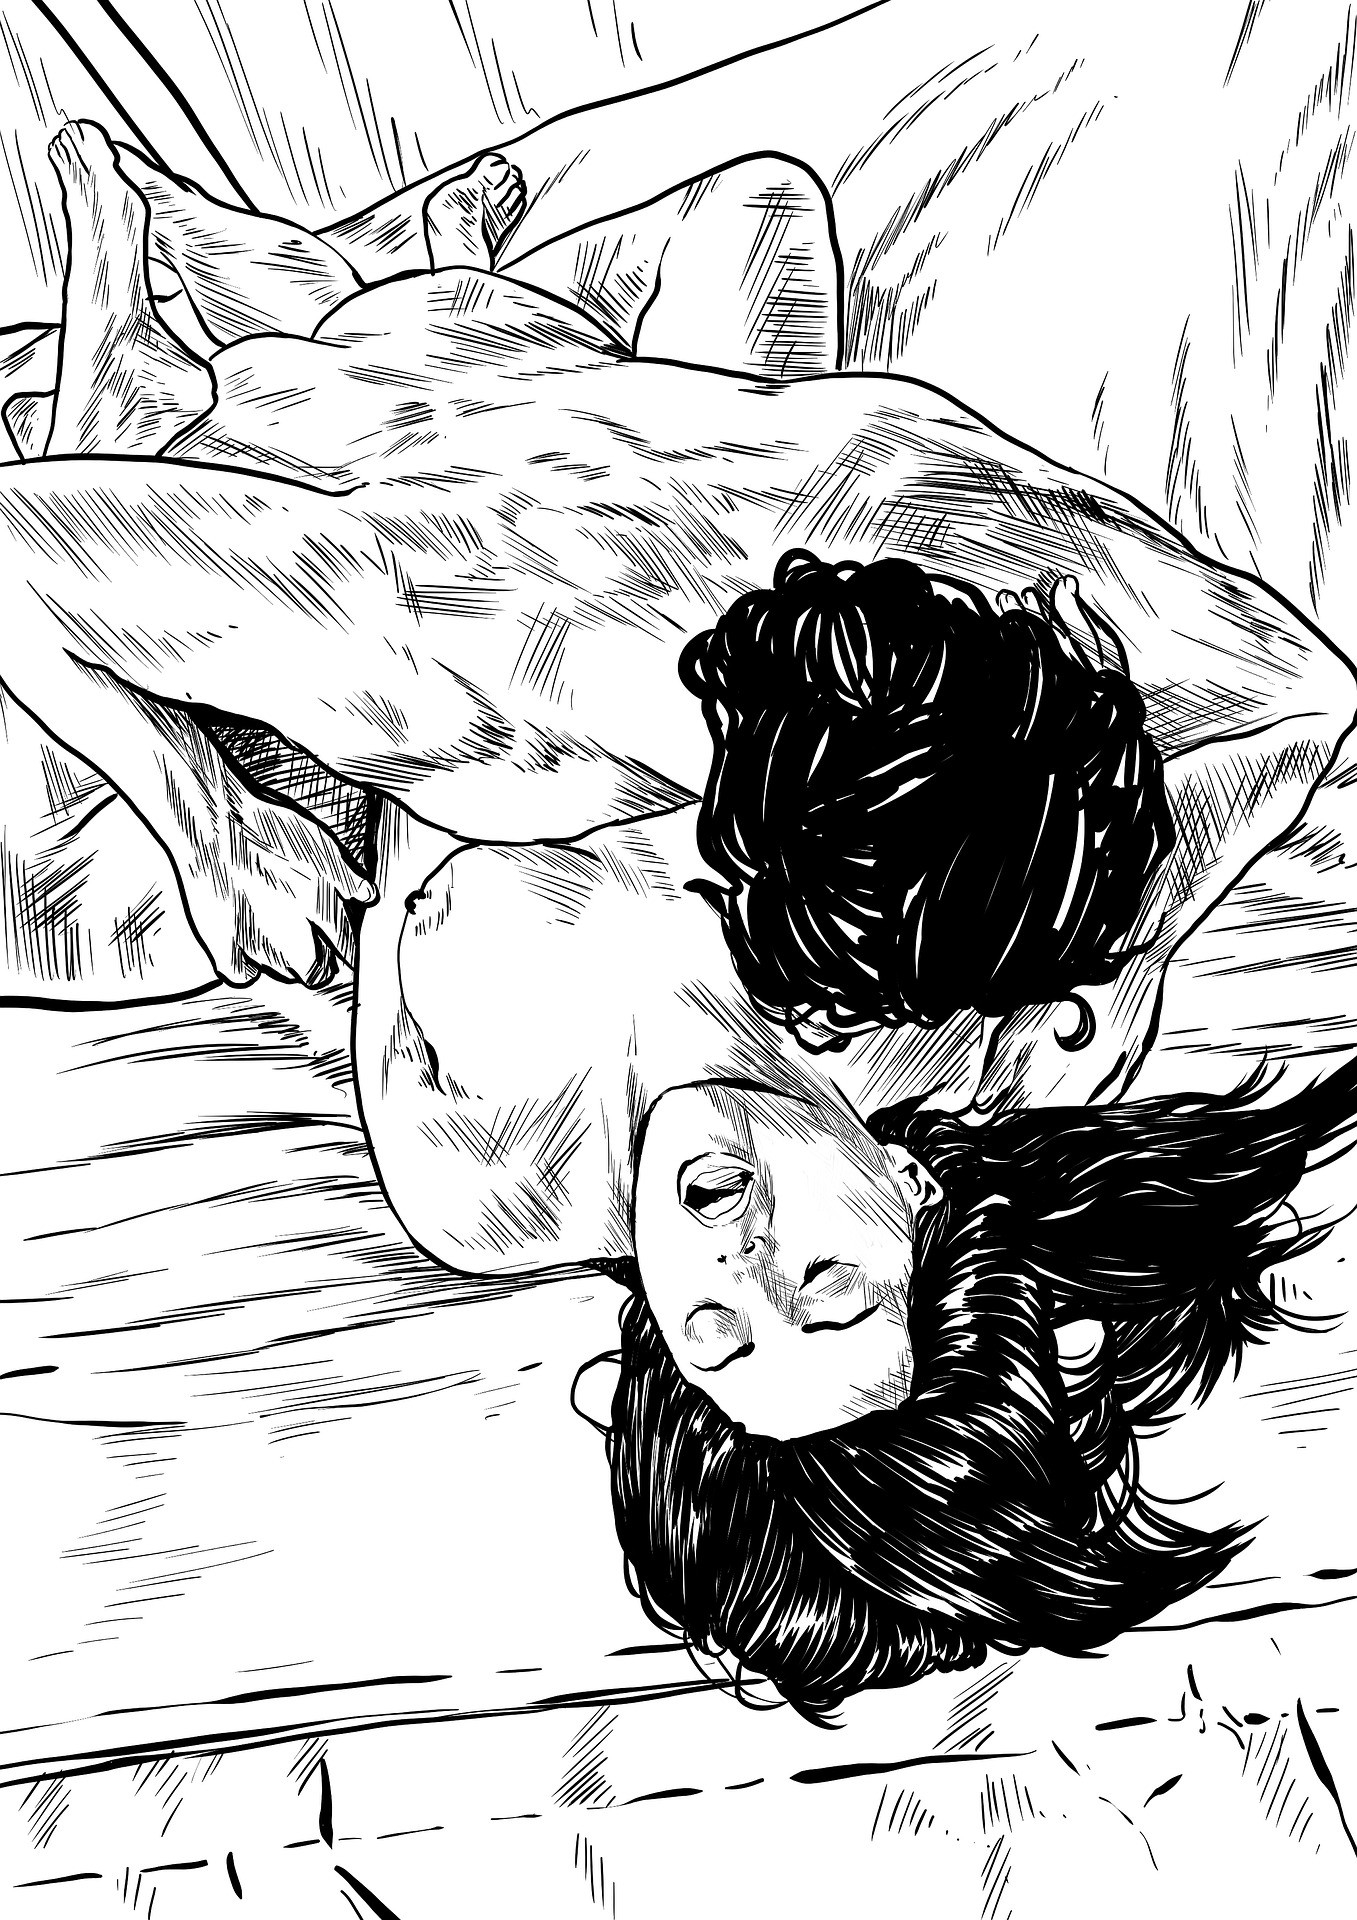
\includegraphics[width=0.7\textwidth]{images/brev73.png}
\end{center}


\breakpage